\chapter{Animating Trees Using Wind Fields Estimated from Motion Capture Data} 
\label{chap:estwindfield}

\noindent
Jie Long and Michael Jones. Estimating wind flow from tree motion using motion capture data.

\begin{abstract}
We present non-rigid motion capture by extracting external forces from motion capture data and then replaying those forces to create animation. We explore this idea in the context of motion capture of natural trees in wind.  Motion of a tree in wind is decomposed into three forces: wind-induced drag, branch elasticity, and damping by the leaves.  Given a model of elasticity and damping, the drag force can be isolated and used to estimate wind velocity.  The extracted velocity field is extended to a larger volume and enriched with a turbulence model.  That wind field can be replayed on a tree model that includes elastic and damping properties to create similar motion. 
\end{abstract}

\section{Introduction}

\begin{figure}
\centering
        \begin{subfigure}[b]{0.30\textwidth}
                \centering
                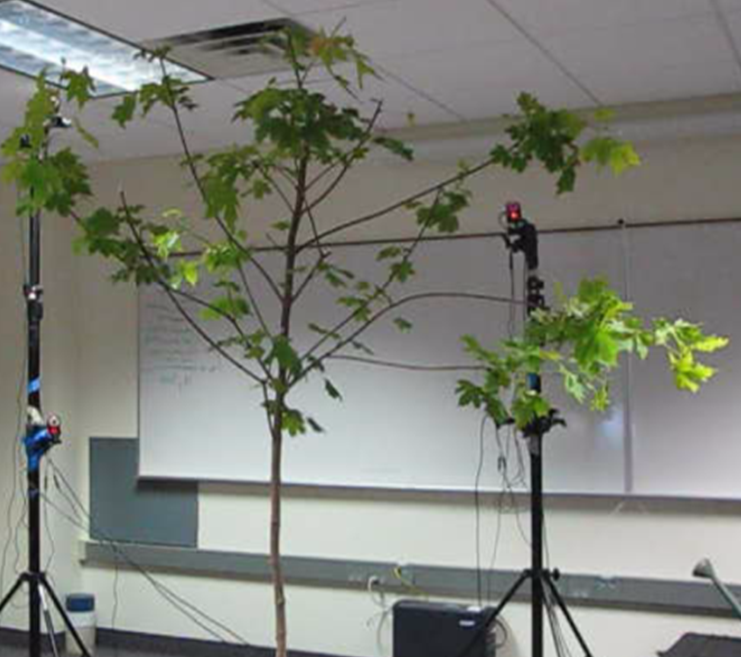
\includegraphics[width=\textwidth]{mocapMaple}
                \caption{Motion capture setup.}
                \label{fig:subfig1}
        \end{subfigure}%
        ~
        \begin{subfigure}[b]{0.3\textwidth}
                \centering
                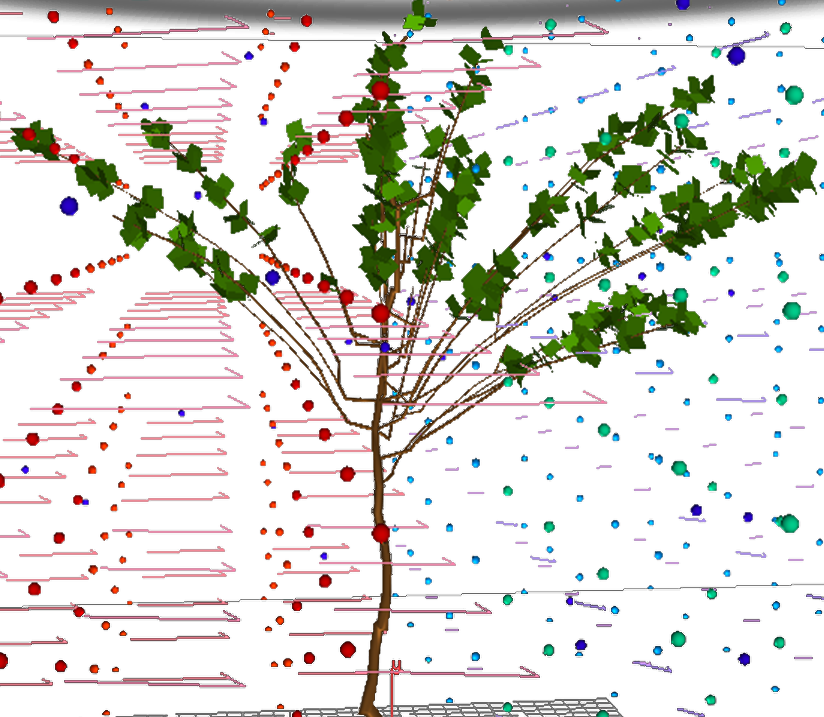
\includegraphics[width=\textwidth]{simulatedField}
                \caption{Extracted wind field.}
                \label{fig:subfig2}
        \end{subfigure}
        ~
        \begin{subfigure}[b]{0.3\textwidth}
                \centering
                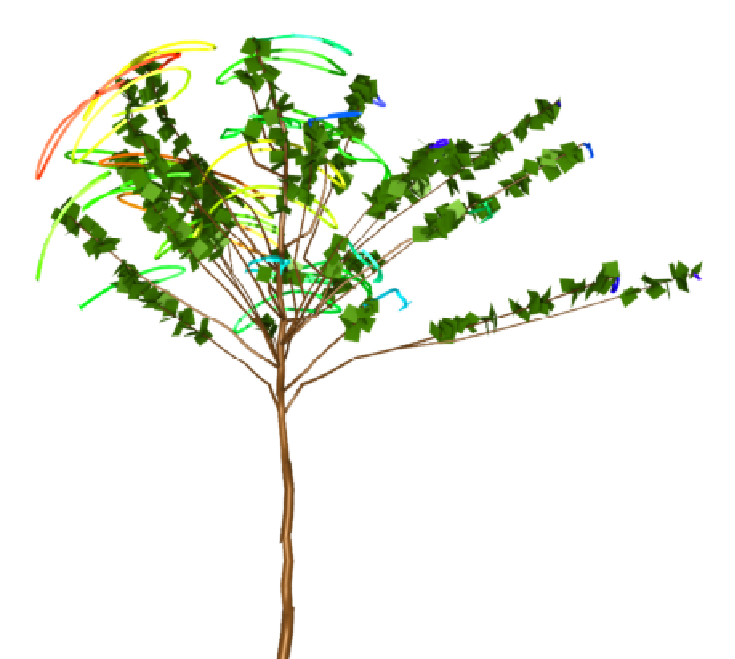
\includegraphics[width=\textwidth]{motionPathMaple}
                \caption{Branch motion paths.}
                \label{fig:subfig3}
        \end{subfigure}        
        \caption[Estimate wind flow and create tree motion. ]{Wind flow can be estimated from motion capture data and used to recreate similar tree motion.}
        \label{fig:title}
\end{figure}

We address the problem of extracting a spatially varying wind velocity field from partial motion captured data and simulating networks of flexible tree branches embedded in a turbulent flow described by this wind field. This problem is a specific instance in which capturing motion and directly replaying it is difficult.  Directly replaying motion capture data is difficult in other settings, such as swimming and rope motion capture, as well.  The problem of replaying tree motion in wind is important for animators and game developers. Tree motion can be an important background element in outdoor settings.  

Animation of trees in wind has been discussed for many years \cite{Akagi:cg06,stams:eu97,shinya:eu92}. In most of the previous research, the wind field is created using noise and fluid simulation. Motion capture avoids the directability and computation problems of simulated wind fields but may yield data that validates simulation-based models.

Motion capture of non-rigid bodies is difficult. Prior work has focused mostly on cloth and facial motion capture \cite{Kwatra:TVCG200966,Ma:FPS2008,SifakisEftychios2005,Lorenzo03}. In these methods, the focus is on overcoming difficulties associated with reconstructing the motion of a deforming plane. We focus on the motion of a deforming network of rods. Rather than directly reconstructing the motion of the deforming object, we reconstruct the forces that create the motion. The forces can then be extended and enhanced to recreate similar motion. 

We solve the problem of extracting a wind field from motion capture data by separating the forces acting on a tree and isolating the force due to wind. There are three primary forces that create tree branch motion: elasticity, damping, and drag. Elasticity and damping can be estimated directly from position and velocity information computed from marker positions. Elastic and damping forces are subtracted from total force to obtain drag. Given drag, we can solve for wind velocity using the aerodynamic drag equation. All of these steps depend on estimates for elasticity, damping, mass, and drag coefficients. These coefficients are estimated from the forestry and graphics literature and can be adjusted to create different motion effects. The extracted wind field has low spatial resolution due to the distances between markers. A sub-grid scale turbulence model with higher resolution restores motion due to omitted high-frequency small-scale turbulence. We use a classical turbulence model composed of a mean flow velocity and turbulence velocity. The mean flow velocity is computed from motion capture data while the turbulence velocity is created using a $tke$ model \cite{Selino:2012,pfa10,pope2000}. The $tke$ turbulence model trains the mean velocity field and modulates tuned noises. By integrating these tuned noises into the wind field, we can restore branches' high-frequency motion while preserving the coherence of branch movements on a tree from large-scale turbulence and small-scale turbulence. 

The process is illustrated in Figure \ref{fig:title}. A tree is instrumented with small retroreflective markers, placed in a passive optical motion capture arena, and subjected to wind. A wind field is extracted, as shown in the middle image. The wind field is applied to a tree model and the resulting motion paths of branch tips are shown in the right-most image.

Our primary contribution is creating complete tree motion from partial motion data collected from motion capture. We discuss methods for sampling and extracting the external force on tree branches as well as energy transformation between tree and wind.

\section{Related Work}

Our work is most closely related to prior work in motion capture of flexible objects and in animating trees. In contrast with prior work in motion capture, we focus on flexible rods rather than flexible planes and on extracting external forces rather than directly extracting motion. In contrast with prior work in animating trees, we estimate a wind field from motion capture data rather than simulating the wind field using noise or approximating it using fluid simulation. 

Motion capture has been widely used in simulating human motion \cite{Kwatra:TVCG200966,Lou:EHM2010,Rajko:2007:RAK,Wen:2006:MCD}. Prior work in motion capture of flexible objects focuses on reconstructing a mesh, which deforms to match a moving surface. Ma et al. \cite{Ma:FPS2008} train a polynomial displacement map and apply this map to create high-resolution facial expressions, including muscle deformation, wrinkles, and skin pores. Lorenzo et al. \cite{Lorenzo03} build a surface-oriented deformation paradigm to animate facial expressions with user intervention. Sifakis et al. \cite{SifakisEftychios2005} combine motion capture data with an anatomical model to produce a model of facial musculature, passive tissue, and the underlying skeletal structure. A key difference between natural trees and facial motion capture is that the drag forces that create natural tree motion in wind may be simpler to extract from motion than the muscular forces involved in facial motion. In this paper, instead of continuously reconstructing a surface, as one does with faces or cloth, we animate trees that have open structures and more degrees of freedom. Also, not only do we create tree motion, but we also simulate wind dynamics, which are scalable.

Recent work extracts forces rather than motion. Kwatra et al. \cite{Kwatra:TVCG200966} simulate human swimming and interaction with water by combining motion capture data and fluid dynamics. Motion capture records swimming motion with an articulated rigid skeleton model. The forces at joints are computed. By combining the forces with fluid dynamics, this method creates human swimming motion as well as water movement. Our research computes wind forces from motion capture data. Compared to Kwatra et al. \cite{Kwatra:TVCG200966}, this would be like capturing the motion of a swimmer in water in order to capture the fluid dynamics around the swimmer. A key difference in our model is that we have assumed that the tree does not initiate motion.

Sun et al. \cite{Sun:2003:VID} propose a method to extract motion patterns from video sequences and reapply these patterns to simulate computer-generated objects. The research focuses on the schema of video input driven animation (VIDA). Motion information is analyzed from 2D video and then incorporated to a conceptual model, such as wind or water dynamics. Our research follows a similar process to the schema. Instead of capturing 2D video, our motion capture system provides more accurate motion information in 3D space. Our research also calculates the interactive energy between trees and wind using particle flow in both space and time domains. By introducing a turbulence model, our tree motion provides more flexibility of simulation control and creates plausible natural tree sway in wind.  

Approaches for simulating tree motion in wind with either one- or two-way coupling in a fluid simulation are based on the Navier-Stokes equations. Akagi \cite{Akagi:cg06} takes this approach but uses a coarse simulation grid, which omits significant high-frequency fluid turbulence. 

The more common approach is to approximate wind dynamics with a frequency-tuned noise model. Ota et al. \cite{ota:cgi03} apply an experimental noise model of ${1/f^\beta}$ to simulate the motion of branches and leaves. Shinya and Fournier \cite{shinya:eu92} present a motion model based on a stochastic process and physical dynamics. They use a power spectrum and autocorrelation of wind to generate a spatiotemporal wind velocity field similar to that created when wind flows through trees. Habel \cite{Habel09PGT} builds a 2D-motion, rather than velocity, texture by combining a Gaussian field with a frequency-tuned 2D velocity field based on a wind dynamics equation with a harmonic oscillator model. The motion texture synthesizes branch motion directly without an integration step. This runs in real time for three moderately complex trees. Stam \cite{stams:eu97} creates filters for white noise and generates wind fields from samplings. He defines and applies the filtering rules in the frequency domain. The noise model with physical dynamics provides control flexibility and works to create motion for complicated large-scale scenes \cite{ZhangSTCP06}. In our research, wind field calculation is driven by branch movements recorded from motion capture. A turbulence model preserves local wind dynamics using particle flow. Using a smooth window, our approach also avoids the complicated time integration of the dynamic system.

Models for simulating large deformation in networks of flexible rods can be applied to animation of trees in wind. Barbic and Zhao \cite{Barbic:2011:RLS} present a scalable method for simulating both internal and external forces that can be applied to trees. If combined with a model of external forces due to wind, this may result in convincing methods for animating trees in wind.  

Tree motion can also be simulated using data from video or motion capture. Diener \cite{Diener:2006} records 2D video and extracts features for a single plant. By analyzing the video with these features using hierarchical retargeting algorithms, the 2D motion is projected into 3D space and animates a large class of virtual shrubs.  Long et al. \cite{Long:MCN2010} reconstruct 3D tree motion in wind using motion capture. Reflective sensor markers are placed along branches. Leaves have to be sparse to ensure the visibility of all markers exposed to capture motion. This approach produces visually realistic movements of a cherry tree in wind. However, this method can only create motion of the original tree and is not scalable to other models. In our research, wind field information is trained from motion capture data. Using particle flows for local wind energy transfer, we are able to simulate the motion of multiple objects in a scene. In addition, reflective markers are placed on the tree crown instead of along a single branch. This design maximizes the visibility of markers to motion capture and records more accurate movement data. It also facilitates the computation with the dynamic model of wind and tree.

\section{Methods}

We estimate a wind field from tree motion using motion capture data.  Natural tree motion is captured using passive optical motion capture.  The data are analyzed to estimate both a 3D model of the tree geometry and a wind field.  The estimated wind field approximates the wind that created the motion recorded in the motion capture data.  A fluid simulation enriched with a synthetic turbulence model transfers energy between wind and tree.  The enriched fluid simulation drives animation of a tree model.  

Our work can be divided into three parts: motion capture, tree modeling, and wind--tree interaction. We describe each part in the following sections. Of those three parts, wind--tree interaction presents the most difficult and interesting problems. 

\subsection{Motion Capture}

As in \cite{Long:MCN2010}, twelve optical motion capture cameras are placed in a circle around a tree indoors. A fan with varying speed and direction creates tree movement. The cameras record the motion of markers placed on exterior branch tips. Placing markers on branch tips avoids problems with occlusion. Typically we use about 30--70 markers, depending on the size and shape of the tree. Markers are distributed evenly to cover the crown shape. 

Optical motion capture records unindexed locations of all the reflective markers in a scene. The recorded data can be processed to label unindexed locations and to eliminate swaps and repair gaps. The algorithm uses forward differences to predict the future position of a point and then minimize the distance between the predicted and the recorded points to add a new position to an existing trace. Details can be found in \cite{Long:MCN2010}. At the end of the process, collected marker positions are clustered into paths for each marker. 

\subsection{Tree Modeling}

Particle flow can generate 3D branching structures \cite{Tan:2007:ITM,neubert:acmtg07,Runions07}. In most cases, this approach depends on inverse volumetric rendering to identify the position of tree mass.  The tree mass is then filled with a branching structure using either particle flow or pre-built libraries of small branching structures.  Motion capture data simplify the process because explicit image segmentation and camera calibration are not needed, as they are part of the motion capture process.  

Particle systems generate the branching structure.  In our process, particles are generated at the 3D positions recorded for the branch tips on which reflective markers were placed. We generate additional particles distributed evenly on the periphery of the region bounded by the tree crown. Each of these particles also represents a branch tip.

\begin{figure}[!t]
\centering
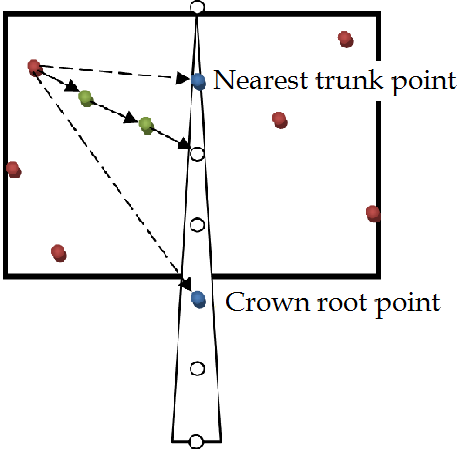
\includegraphics[width=1.8in]{particle}
\caption{A particle with its nearest trunk point and its crown root point.}
\label{fig:particle}
\end{figure}

The particles flow toward a predefined trunk placed vertically in the center of the crown shape. Branch shapes and hierarchies are defined when particle paths connect. Particle flow starts at branch tips and ends at the trunk. Each particle has a direction, a step length, and a threshold for merging. As in \cite{neubert:acmtg07}, the particle direction combines the direction to the crown root point and to the nearest trunk point, shown in Figure \ref{fig:particle}. The red dots in the image indicate locations of branch tips. The crown root point is the lowest point on the trunk near the bounding box of tree crown. The nearest trunk point is on the trunk that has the shortest distance toward a particle. Particles flow from branch tip toward the trunk, which is unlike the particle system in \cite{palubicki:siggraph09}, where particles flow from trunk to branch tip. The direction of the first step in the flow is the combination of direction to the nearest trunk point and the crown root point. In the following steps, the flow direction is also a combination of these two directions, but any two particles are merged if their distance is under the threshold of merging distance.

\subsection{Wind--tree Interaction}

Wind--tree interaction is based on a mixed Lagrangian/Eulerian model of the wind field extracted from motion capture data enriched with a subgrid turbulence model. The Eulerian grid stores wind velocities as estimated from motion capture data. Lagrangian particles carry velocity and turbulent kinetic energy $tke$ from frame to frame. The \textit{velocity grid} is replaced every frame while the \textit{fluid particles} retain state from frame to frame.
Fluid particles carry energy back and forth between the global wind field, the local turbulence model, and the tree. In this way we simulate tree movement as well as the distribution of energy in a dynamic wind velocity field.

Proxy geometry is used to detect and approximate the effects of collisions between fluid particles and tree geometry. Both the effect of wind on trees and the effect of the tree on wind are calculated.  

Because the global velocity field is generated from motion capture data, which may contain noise, this field may not be continuous in the time domain. Averaging velocity values for a single grid across several adjacent frames smoothes these variations but also smoothes small-scale turbulence effects. In order to compensate for lost turbulence effects as well as to better preserve wind continuity over time, particles store $tke$ across frames and manipulate the scale of turbulence due to characteristics of tree and wind. 

\subsubsection{Wind Velocity Field}

The global grid-based velocity field is the source of wind energy in the scene. Wind force is estimated directly from recorded displacements of branch tips. We solve for wind velocity at branch tips using drag equations and the estimated wind force.  This gives a sparse collection of velocity estimates.  Interpolation and extrapolation build a grid of velocity values from the sparse collection. Figure \ref{fig:vectorField} shows an orthographic projection of such a field. The green dots indicate marker positions, the red arrows represent extracted wind velocities, and the blue arrows represent velocities interpolated or extrapolated from the estimated velocities. The wind field in Figure~\ref{fig:vectorField} is quite smooth.  This is because small-scale turbulent eddies are below the spatial sampling resolution of the motion capture data.  A subgrid turbulence model based on $tke$ recreates small eddies in the velocity field. 

\begin{figure}[!t]
\centering
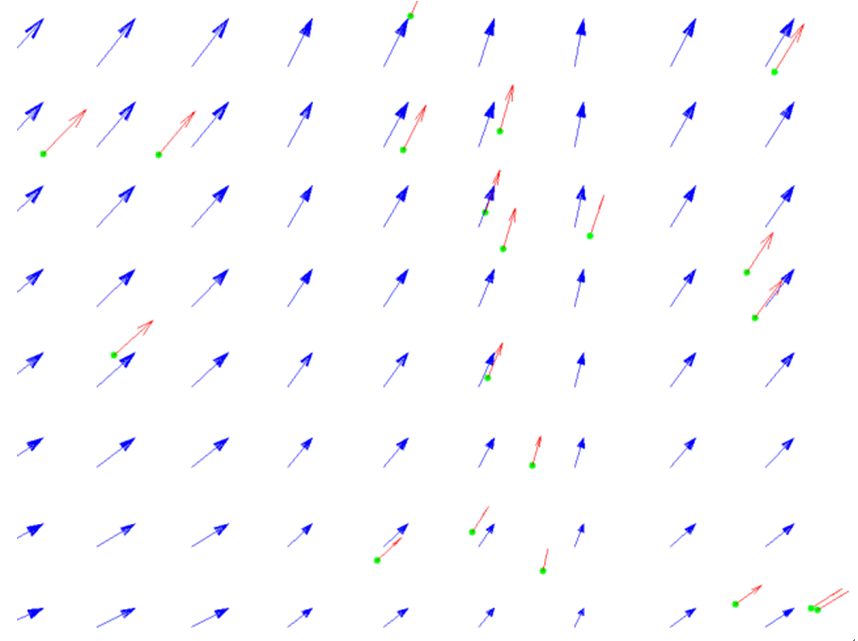
\includegraphics[width=2.5in]{vectorField}
\caption{Vector field of wind velocities with estimated and interpolated values. Wind velocity estimates based on recorded tree motion are shown in red with interpolated velocities in blue.}
\label{fig:vectorField}
\end{figure}

We isolate the drag force in order to estimate the wind velocity.  Assuming no external forces other than wind influence the tree motion, the motion of a branch is caused by aerodynamic drag and internal elasticity and damping forces. Elastic forces tend to restore the branch to a resting position and damping forces reduce velocity. In this model, the forces acting on a tree are given by 

\begin{equation}
\label{eqn:1}  
			F = F_{wind} + F_{elastic} + F_{damping} = F_{wind} + c\dot{s} + ks.
\end{equation} 

Differences between marker positions in successive frames give estimates for position $s$, velocity $\dot{s}$ and acceleration $\ddot{s}$. All the derivatives are approximated with the marker positions using backward differencing. The displacement $s$, velocity $\dot{s}$ and acceleration $\ddot{s}$ are calculated as

\begin{equation}
\label{eqn:diff}
s^t = q^t - q^{t-1},\\
\dot{s}^t =  (s^t - s^{t-1})/2.0,\\
\ddot{s}^t = (\dot{s}^t - \dot{s}^{t-1})/2.0,
\end{equation}
where $q^t$ is a marker position at time $t$. The elastic force $F_{elastic}$ is the product of branch elasticity and displacement from the rest position. Similarly, the damping force is the product of the damping coefficient and the velocity. We estimate damping $c$ and spring coefficients $k$ from biomechanical parameters. Since $F = m\ddot{s}$, we substitute $m\ddot{s}$ for $F$, make similar substitutions for the elastic and damping forces, and then solve for $F_{wind}$ to obtain 

\begin{equation}
\label{eqn:2}
			F_{wind} = m\ddot{s} - c\dot{s} - ks.      
\end{equation}

The drag equation gives the force created by wind as a function of the wind velocity $V$ (and other constant parameters explained below): 

\begin{equation}
\label{eqn:3}
			F_{wind} = 0.5\rho(V^2)AC_D,
\end{equation}
where $\rho$ is air density, $V$ is wind velocity relative to branch movement, $A$ is the aerodynamic cross section, and $C_D$ is the drag coefficient.

Substituting the value of $F_{wind}$ calculated using equation (\ref{eqn:2}) into equation (\ref{eqn:3}) and solving for $V^2$ gives

\begin{equation}
\label{eqn:4}
		V = \frac{F_{wind}}{\left\|F_{wind}\right\|} * \sqrt{\left|\frac{m\ddot{s} - c\dot{s} - ks}{0.5{\rho}AC_D}\right|}.
\end{equation}

The solution is based on the assumption that the acceleration is constant and therefore the direction of velocity $V$ and force $F_{wind}$ is preserved as the same in a short period of time. In our case, the time interval is 0.01 sec from motion capture setup. The direction of the velocity $V$ is computed using the unit normal vector of $F_{wind}$ as shown in equation (\ref{eqn:4}). The displacement $s$, velocity $\dot{s}$ and acceleration $\ddot{s}$ are computed using equation (\ref{eqn:diff}) from the marker locations.

The equation (\ref{eqn:4}) calculates a wind velocity estimate in each frame at the location of each branch tip.  Motion capture markers are distributed evenly through the crown in order to sample the global wind field over a large area. 

Interpolating and extrapolating velocity values over the entire motion capture volume results in a grid-based velocity field. The size of a grid cell is set to be close to the average distance traversed by a single marked branch. By doing this, we can optimize the usage of motion capture data during the interpolating and extrapolating process. In each frame, the ideal case is that each grid cell contains exactly one motion-captured point. In our case, the grid resolution is $10*10*10$. We use linear interpolation to fill the grid from sampled values because linear interpolation is simple.  More sophisticated methods, such as Kriging (as in \cite{ganz:cvpr09}) or distance-weighted kernel-based methods, could also be used.

The grid-based wind velocity field is computed from each individual frame of branch tip data. However, the wind velocity field does not vary smoothly from frame to frame because there are gaps and jumps in the data. To improve temporal continuity, velocity values over the neighboring 5 frames are averaged. 

Turbulent motion below the sampling scale of the motion capture data cannot be captured by this model. In space, we are only able to extract turbulent effects that are large enough to influence the motion of two adjacent markers. Because leaves have small mass and large surface area, small-scale turbulence results in visually significant motion on tree crowns. That turbulence is well below the sampling limit of the data. The mean flow inferred from motion capture data will be enriched with a turbulence model at a finer resolution. 

Rather than apply the velocity field directly to the tree, we introduce particles into the field and collide particles with proxy spheres attached to the tree. These particles have zero mass and do not affect the mean flow. This scheme simplifies calculation of wind--tree interaction by replacing cell--tree collisions with point--sphere collisions. Cell--tree collisions can be expensive for determining what fraction of a cell contains a fraction of a generalized cylinder representing the tree branch. With particles and proxy geometry, estimating wind velocity can be reduced to a distance-weighted average of the particles contained in a sphere. 

\subsubsection{Wind Effects on a Tree}
%why we use the approach? motivation
Simulating wind effects on a tree creates branch motion. The simulation is the key to creating natural tree motion. We have discussed creating a grid-based wind velocity field using motion capture data. Because of motion capture's capability to record a limited number of markers, the resolution of the gird is low. The low resolution simulates big-scale turbulence but lacks small-scale turbulence information due to a high-frequency wind field. Selino and Jones \cite{Selino:2012} solve this problem by introducing the small-scale turbulence, which is computed from large-scale turbulence. This solution fits into our problem very well. In our case, the low resolution of the wind velocity field produces large-scale turbulence. The large-scale turbulence will be tuned by a $tke$ model to create small-scale turbulence. The combination produces wind effects, including both large- and small-scale turbulence, on a tree.

% a summary of the approach. 
The simulation of wind effects on a tree preserves coherence of velocity from several perspectives. The mean flow velocity computed from interpolating motion capture data contains information of tree movements as a whole. The $tke$ model keeps track of turbulence changes in the flow and thus tunes the noise value due to these changes. The Gaussian noise field is filtered in the frequency domain to match the frequency of turbulence observed in tree crowns. The model is derived from a classical turbulence model and generates turbulence effects, including both large scale and small scale.

%How does our method work?
Our approach is different from Selino's work because of the source of large-scale turbulence. Instead of a real-time fluid simulation, we generate the large-scale turbulence offline from motion capture. In Figure \ref{fig:turbulenceFlow}, we demonstrate our turbulence model to generate tree motion. The turbulence is computed in two parts as in large scale and small scale. The large-scale turbulence is created from the grid-based wind velocity field. The small scale is generated from the $tke$ model. After solving the turbulence velocity, we apply a drag equation as shown in equation (\ref{eqn:3}) to solve for the tree motion represented by branch displacements. 

\begin{figure}[!t]
\centering
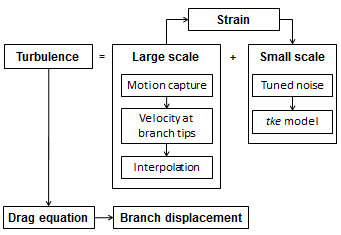
\includegraphics[width=3.4in]{turbulenceFlow}
\caption{Turbulence simulation to create branch motion.}
\label{fig:turbulenceFlow}
\end{figure}

% the basic equation
The turbulence velocity $V(t)$ applied to a branch segment is computed as in equation (\ref{eqn:5}):

\begin{equation}
\label{eqn:5}
		V(t) = v(t)+ \alpha\sqrt{k(t)}N(t),
\end{equation}
where $v(t)$ is the mean flow velocity for the large-scale turbulence at time $t$, $\alpha$ is a tunable weight parameter, $k(t)$ is from $tke$ model, and $N(t)$ is a sampled value from a frequency-tuned time-varying noise field. 

%explain $tke$ tuned high frequency velocity component
In the simulation, each fluid particle carries a mean flow velocity from the global wind velocity field and a $tke$ estimate from the turbulence model. The value $k(t)$ of the $tke$ is estimated using a two-equation $tke$ budget based on strain in the velocity field as shown in equation (\ref{eqn:tkeProduction}) and (\ref{eqn:tkeProductionZero}). The $tke$ model is adapted from Selino \cite{Selino:2012} and Pfaff et al. \cite{pfa10}, and is based on Pope \cite{pope2000}. The value $k(t)$ represents turbulent kinetic energy and is generated when the strain in the mean flow velocity is not zero. The decay term $\epsilon$ models dissipation rate of that turbulence energy. When the turbulence production $P$ exists due to strain, the $k$ and $\epsilon$ are computed as follows:

\begin{equation}
\label{eqn:tkeProduction}
		\frac{\partial{k}}{\partial{t}}=P-\epsilon, 
		\frac{\partial{\epsilon}}{\partial{t}}=C_{\epsilon1}\frac{P\epsilon}{k}-C_{\epsilon2}\frac{\epsilon^2}{k},
\end{equation}
where $P$ is the production of turbulence, $t$ is current time step, and model constants are $\epsilon1$ = 1.44 and $\epsilon2$ = 1.92. When the production $P$ of turbulence in the fluid becomes zero, the values of $k$ and $\epsilon$ dissipate and compute as in the equation (\ref{eqn:tkeProductionZero}):

\begin{equation}
\label{eqn:tkeProductionZero}
	k(t) = k_0\left(\frac{t}{t_0}\right)^{-n}, 
	\epsilon(t) = \epsilon_0\left(\frac{t}{t_0}\right)^{-(n+1)},
\end{equation}
where $t$ is current time step, $n$ is a constant decay component computed by $\frac{1}{C_{\epsilon2-1}}$, $k_0$ and $\epsilon_0$ are the most current values, respectively, in the past when there exists turbulence production $P$, and the reference time $t_0$ is computed as $n\frac{k_0}{\epsilon_0}$.

Based on equation (\ref{eqn:tkeProduction}) and (\ref{eqn:tkeProductionZero}), we compute for the value of $k(t)$ in equation (\ref{eqn:5}).

The noise $N(t)$ is sampled from a continuous noise field. That noise field is tuned to match the frequency distribution of turbulent flow through trees given in Simiu \cite{simiu1996wind}.

%explain mean flow velocity
The mean flow velocity $v(t)$ is sampled using a distance-weighted average of particles' velocity contained within the proxy sphere of a branch tip. Proxy geometry is defined for each branch segment using 3D spheres with radii proportional to branch segment length and diameter as suggested from Selino and Jones \cite{Selino:2012}. 

% a bigger picture
Figure \ref{fig:flowChart} shows the energy flow during the simulation. Wind energy is transferred from the grid-based velocity field to particles. The turbulence model calculates $tke$ from the transferred wind energy. When particles pass through proxy geometry, velocity is converted to a drag force using equation (\ref{eqn:3}) and branch motion is created. 

\begin{figure*}[!t]
\centering
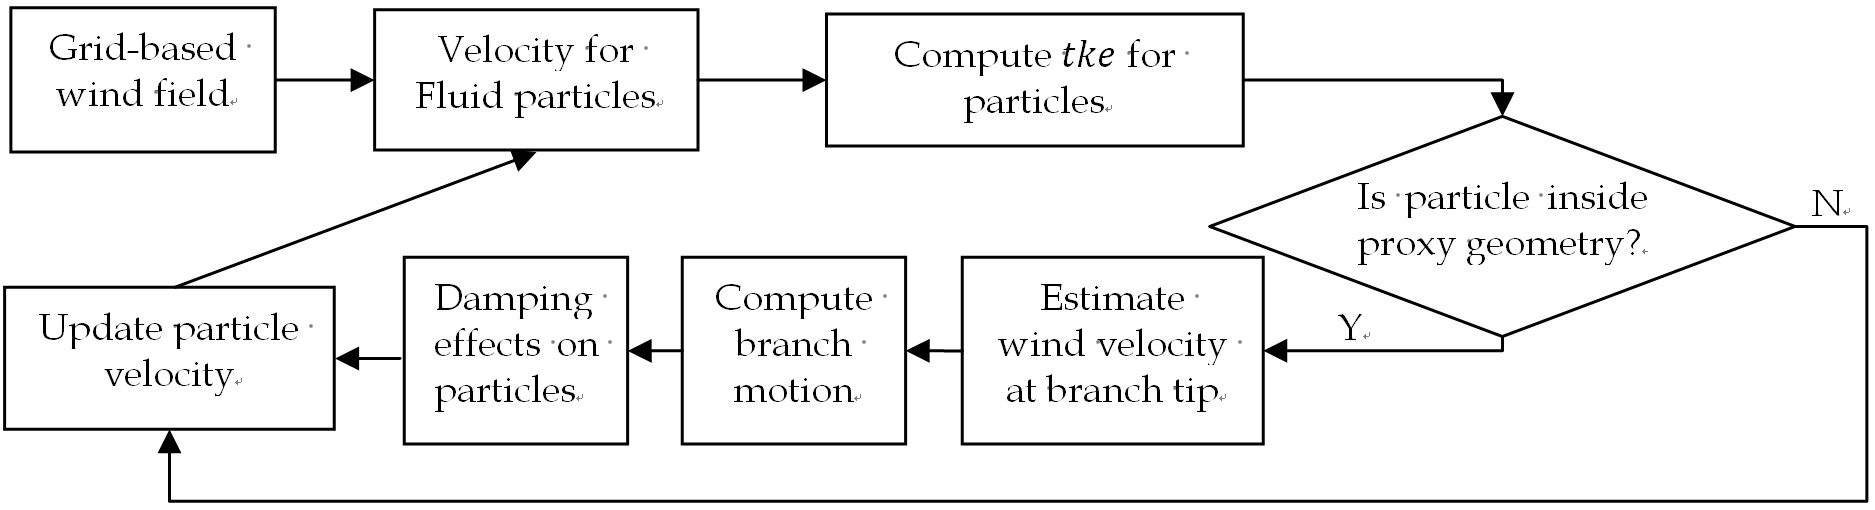
\includegraphics[width=6in]{energyFlow}
\caption{Energy flow in a wind velocity field.}
\label{fig:flowChart}
\end{figure*}

\subsubsection{Tree Effects on Wind}

Tree effects on wind are split into local and global effects. Local effects happen at the scale of a few leaves and branch segments.  Global effects happen at the scale of the entire tree.  Local effects are simulated using a simple damping model on wind particles, and global effects are recorded during motion capture.  Simulating local effects allows for variations in wind flow due to differences between the shape and dynamics of the animated tree compared to the shape and dynamics of the actual tree used in motion capture. 

Tree effects on wind on the local scale are calculated as a damping force for particles within the proxy geometry representation of tree mass. Consider the velocity $v_i(t)$ of particle $i$ in frame $t$  sampled before calculating branch movement. Suppose that particle $i$ lies in proxy geometry for some branch in frame $t$. After displacement of the branch tip has been calculated, if the particle lies within the proxy geometry then we compute the influence of the branch on the particle velocity. The new velocity of particles in the proxy geometry is computed as follows in equation (\ref{eqn:6}):

\begin{equation}
\label{eqn:6}
		v_i^{'}(t) = v_i(t)(1-\beta),
\end{equation}
where $\beta$ is a constant decay rate that changes particle velocity based on damping by the tree. The rate is constant for each branch, but varies due to the size, material, leaf shapes, and other properties of the tree. We set the reduction rate between 0.02 and 0.05 in most simulations. This reduction smoothes out the mean velocity over time while the high-frequency details are compensated from the $tke$ turbulence model.

In the next frame $t+1$, we first load the estimated global grid-based wind field generated from motion capture data. The particle velocity $v_i^{'}(t)$ from the previous frame is used as the mean flow velocity to compute the current particle's turbulent kinetic energy $k(t+1)$. Then we use equation (\ref{eqn:4}) to calculate wind velocity $V(t+1)$ experienced by the tree geometry. 

The global effect of the tree on the wind is inferred from the motion capture data. Branches on the leeward side of the tree have less motion. When the particle exits the proxy geometry, the damping is no longer computed, so the particle velocity is reset to match the estimated global velocity $v$.

\subsubsection{Tree Animation}

The movement of the whole tree is computed from the drag force at each branch tip. We use a damped mass-spring model to define branch dynamics. When the density, stiffness, and damping coefficients match the estimates used to calculate wind velocity, the resulting motion is similar to the original motion. The drag forces are calculated for each branch segment.

\section{Results}
\label{sec:4results}

We present results that show animation of a tree in wind using a wind velocity field inferred from motion capture data for a similarly sized tree moving in wind.  

We first create a 3D tree shape using particle flow. In Figure \ref{fig:treeshape}, the small white cubes on some of the branch tips indicate the location and total number of reflective markers we capture for the tree. The locations of branch tips that do not correspond to a marker location are created within the stacked bounding boxes. We generate tree leaves based on the branching structure and instance leaf size and shape randomly. By the refined bounding box method, the generated 3D tree shape also is visually similar to the crown shape of the original tree. The similarity between the generated tree model and the actual tree shape can be seen in parts (a) and (b) of Figure~\ref{fig:title}.  It is significant that the tree shape does not perfectly match the original tree shape.  Applying the motion capture data indirectly as an inferred wind velocity field, rather than directly as a set of motions, allows for variations in tree shape and branching structure.  

\begin{figure}[!t]
\centering
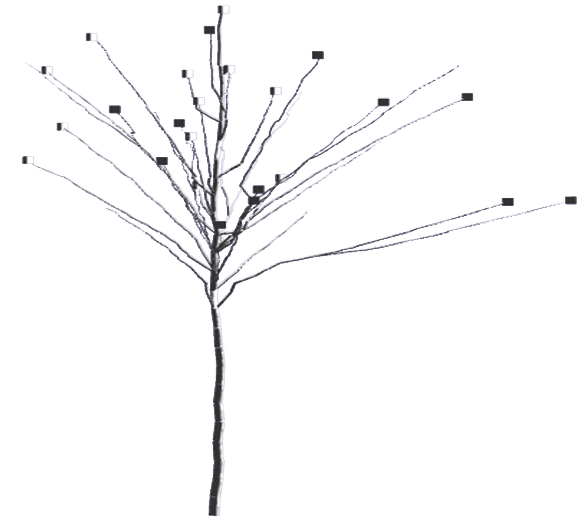
\includegraphics[scale=0.5]{mapleModelMocapTip}
\caption{3D branching structure with marker locations.}
\label{fig:treeshape}
\end{figure}

The $tke$ model is a significant part of producing realistic motion. In Figure \ref{fig:branchPath}, we compare the results generated with and without turbulent $tke$. Each figure shows motion paths from an animation of a tree in wind with and without sub-grid turbulence based on the $tke$ model.  The path on the left includes motion due to sub-grid $tke$ and the path on the right does not.  In both cases, moving branches trace out arcs of similar size as they sway left and right.  Adding $tke$ has the effect of adding variation to each sway motion so that the arcs are each in a slightly different location.  As a result, the motion path on the left, which includes $tke$, is less compact while the motion path on the right, which does not include $tke$, contains many overlapping arcs.

\begin{figure}[!t]
\centering
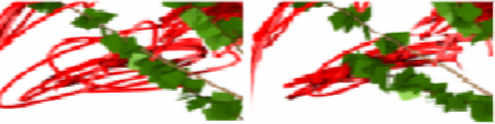
\includegraphics[scale=0.6]{branchPath}
\caption[Branch motion paths with and without subgrid turbulence.]{Branch motion paths with (left) and without (right) sub-grid turbulence. Adding turbulence adds small variations to each branch sway, as seen in the less compact motion path on the left.}
\label{fig:branchPath}
\end{figure}

The images in Figure \ref{fig:motionPaths}\subref{fig:branchTipMocap} and \ref{fig:motionPaths}\subref{fig:branchtipSynthesized} compare recorded motion of a tree with motion generated for a similar tree using the wind field inferred from motion capture data.  The actual tree motion is shown using green traces on the left and the generated motion is shown on the right.  Note that motion is not captured for every branch tip on the left, but motion is generated for every branch tip on the right.  The images have been aligned so that the wind direction is the same in both cases.  Branches in similar positions on the crown have similar motion. 

\begin{figure}
\centering
        \begin{subfigure}[b]{0.29\textwidth}
                \centering
                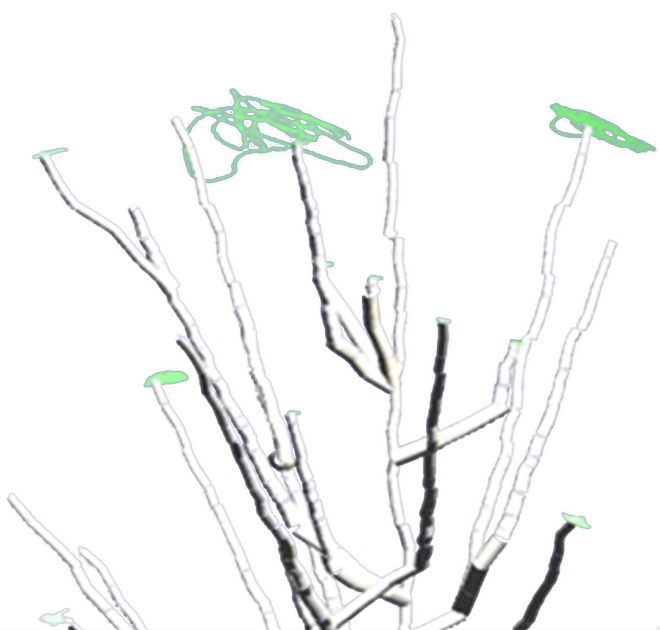
\includegraphics[width=\textwidth]{branchTipMocap}
                \caption{Original tree motion.}
                \label{fig:branchTipMocap}
        \end{subfigure}%
        ~
        \begin{subfigure}[b]{0.3\textwidth}
                \centering
                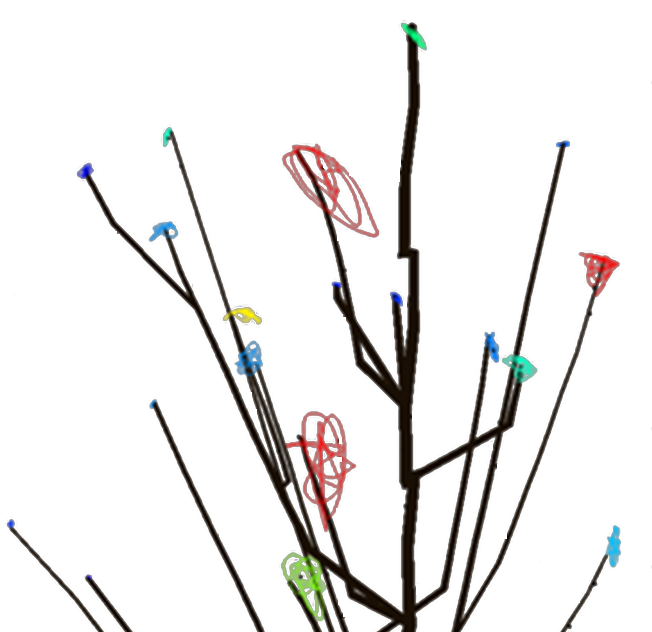
\includegraphics[width=\textwidth]{branchtipSynthesized}
                \caption{Animated tree motion.}
                \label{fig:branchtipSynthesized}
        \end{subfigure}       
        \caption[Motion paths for the animated tree. ]{Motion paths for the animated tree are similar to motion paths in the original tree for branch tips at the same relative crown location.}
        \label{fig:motionPaths}
\end{figure}

In Figure \ref{fig:mapleSway}, we demonstrate that our method produces plausible tree sway motion and results in tree motion effects observed in nature, such as sheltering.  Branches bend with the wind and then return to their rest position.  Branch sheltering within a single tree crown occurs when branches on the leeward side of the crown experience lower wind velocities than branches on the windward side because drag exerted by the windward branches reduces the wind velocity.  In the figure, the dominant wind direction is from left to right and from the lower left corner. We can observe that branches, which are on the left side (the windward side), have bigger amplitude of motion than others. Besides completing tree motion of a single similar tree with partial motion capture data, our method can also be extended to create tree motion for multiple trees using the wind field.  The trees in Figure \ref{fig:multipleTrees} move in the same wind field.  Although this creates the appearance of a group of trees moving in a shared environment, wind is not damped as it passes from one tree to another.  In the video clip attached to this paper, we provide a side-by-side comparison of the video originally recorded during the motion capturing process and the synthesized tree animation. From the video, we can observe that sheltering effects among branches are successfully simulated. 

\begin{figure*}[!t]
\centering
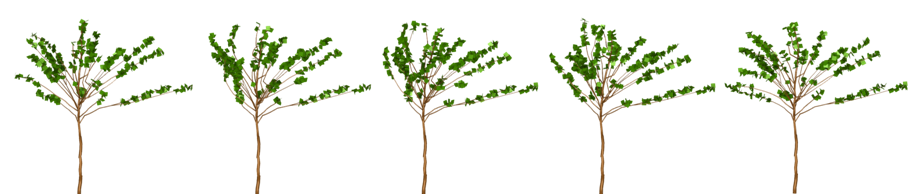
\includegraphics[scale=0.65]{mapleSway}
\caption[Maple animation.]{Several frames from the animation of a maple tree in a wind field extracted from motion capture data.}
\label{fig:mapleSway}
\end{figure*}

\begin{figure}[!t]
\centering
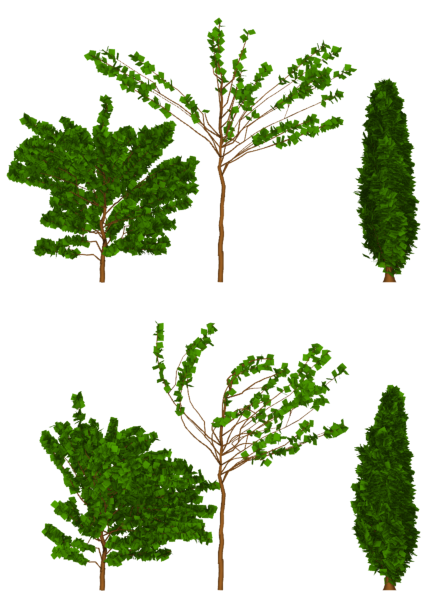
\includegraphics[scale=0.68]{multipleTrees}
\caption[Multiple trees swaying. ]{Multiple trees swaying in wind field estimated from the motion of a single tree.}
\label{fig:multipleTrees}
\end{figure}

\section{Discussion and Future Work}

We have presented animation of non-rigid bodies using partial motion capture data by extracting a wind velocity field rather than replaying motion data directly. This simplifies the problem as we no longer need to match motion capture data to a precise reconstruction of the original capture subject. It also results in complete and coherent motion from incomplete data that contains discontinuous motion. We have also presented a method for enriching the extracted force field to include fine-resolution turbulence. This is possible because the extracted velocity field can be analyzed and enriched, much like position graphs can be analyzed and enriched in other applications.  

This work opens a new direction in the motion capture of non-rigid bodies in spatially smooth force fields. We have investigated this idea in the context of trees and wind. Future work might focus on other objects, such as cloth, in other flows.